\documentclass[letterpaper]{deedy-resume} % Use US Letter paper, change to a4paper for A4 
\usepackage{fontawesome}
\usepackage{tikz}

\begin{document}

%----------------------------------------------------------------------------------------
%	TITLE SECTION
%----------------------------------------------------------------------------------------

\lastupdated % Print the Last Updated text at the top right

\namesection{Justin T.}{Krumlauf}{ % Your name
\urlstyle{same}\url{http://justinkrumlauf.me} \\ % Your website, LinkedIn profile or other web address
\href{jtkrumlauf@gmail.com}{jtkrumlauf@gmail.com} | 203-273-1386 % Your contact information
}

%----------------------------------------------------------------------------------------
%	LEFT COLUMN
%----------------------------------------------------------------------------------------

\begin{minipage}[t]{0.33\textwidth} % The left column takes up 33% of the text width of the page

%------------------------------------------------
% Education
%------------------------------------------------

\section{Education} 

\subsection{Rochester Institute \newline
of Technology}

\descript{Computing Security Major}

\sectionspace % Some whitespace after the section

%------------------------------------------------
% Links
%------------------------------------------------

\section{Links} 

\faGithub:  \href{https://github.com/jtkrumlauf}{\bf jtkrumlauf} \\
\faLinkedin: \href{https://www.linkedin.com/in/jtkrumlauf}{\bf jtkrumlauf} \\
Website: \href{justinkrumlauf.me}{\bf justinkrumlauf.me} \\

\sectionspace % Some whitespace after the section

%------------------------------------------------
% Coursework
%------------------------------------------------

% \section{Coursework}

%------------------------------------------------

% \subsection{Undergraduate}

% Cool Stuff \\
% Some more cool stuff \\
% even cooler stuff

% \sectionspace % Some whitespace after the section

%------------------------------------------------
% Skills
%------------------------------------------------

\section{Skills}

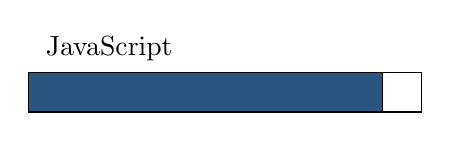
\begin{tikzpicture}
\node [anchor=west] at (.1,.8) {JavaScript};
\draw [fill=white] (0,0) rectangle (5,.5);
\draw [fill={rgb:red,1;green,2;blue,3}] (0,0) rectangle (4.5,.5);
\end{tikzpicture}

\vspace{.05cm}
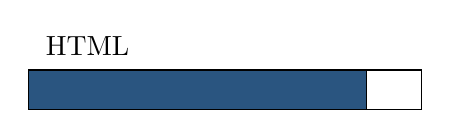
\begin{tikzpicture}
\node [anchor=west] at (.1,.8) {HTML};
\draw [fill=white] (0,0) rectangle (5,.5);
\draw [fill={rgb:red,1;green,2;blue,3}] (0,0) rectangle (4.3,.5);
\end{tikzpicture}

\vspace{.05cm}
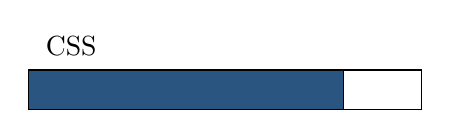
\begin{tikzpicture}
\node [anchor=west] at (.1,.8) {CSS};
\draw [fill=white] (0,0) rectangle (5,.5);
\draw [fill={rgb:red,1;green,2;blue,3}] (0,0) rectangle (4,.5);
\end{tikzpicture}

\vspace{.05cm}
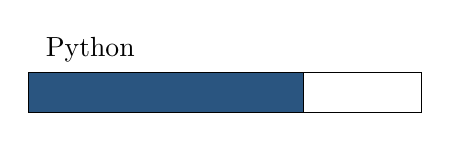
\begin{tikzpicture}
\node [anchor=west] at (.1,.8) {Python};
\draw [fill=white] (0,0) rectangle (5,.5);
\draw [fill={rgb:red,1;green,2;blue,3}] (0,0) rectangle (3.5,.5);
\end{tikzpicture}

\vspace{.05cm}
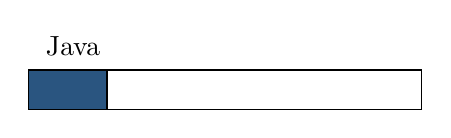
\begin{tikzpicture}
\node [anchor=west] at (.1,.8) {Java};
\draw [fill=white] (0,0) rectangle (5,.5);
\draw [fill={rgb:red,1;green,2;blue,3}] (0,0) rectangle (1,.5);
\end{tikzpicture}


\sectionspace % Some whitespace after the section

%----------------------------------------------------------------------------------------

\end{minipage} % The end of the left column
\hfill
%
%----------------------------------------------------------------------------------------
%	RIGHT COLUMN
%----------------------------------------------------------------------------------------
%
\begin{minipage}[t]{0.66\textwidth} % The right column takes up 66% of the text width of the page

%------------------------------------------------
% Experience
%------------------------------------------------

\section{Experience}

\runsubsection{The Greenwich Country Day School}
\descript{| Teaching Intern}

\location{Nov 2017 - Dec 2017 | Greenwich, CT}
\vspace{\topsep} % Hacky fix for awkward extra vertical space
\begin{tightitemize}
\item Worked alongside faculty in creating the computer science curriculum
\item Helped students design and create projects in the Innovation Lab (Raspberry Pi's, Arduino, 3D Modeling, Computer Aided Design, Websites, etc.)
\item Taught several computer science classes the basics of PyAutoGUI and other Python tools.
\end{tightitemize}

\sectionspace % Some whitespace after the section

%------------------------------------------------

\runsubsection{The Greenwich Country Day School}
\descript{| Tech. Intern}

\location{Mar 2016 – May 2016 | Greenwich, CT}
\begin{tightitemize}
\item Helped teachers with any tech problems they should have
\item Did regular maintenance on 3D printers (Ultimaker Extended, Makerbot, LulzBots)
\item Configured new computers and ensured they were ready for use
\end{tightitemize}

\sectionspace % Some whitespace after the section

%------------------------------------------------

\runsubsection{Local Live TV}
\descript{| Video Producer}

\location{Feb 2014 – Present | Stamford, CT}
\begin{tightitemize}
\item Involved in back-end filming and producing of events
\item Wirelessly film a myriad of High School events such as Ice Hockey, Lacrosse, Theatre and Football
\item Created highlight clips that were then sent off to the respective school
\end{tightitemize}

\sectionspace % Some whitespace after the section

%------------------------------------------------
% Research
%------------------------------------------------

\section{Personal Projects}

\runsubsection{\textbf{\href{http://www.justinkrumlauf.me}{Personal Website}}}
\descript{| Lead Full-Stack Developer}

\location{Sept 2018 – Present | Rochester, NY}
My goal was to create a website where people could come to learn about me and what I do. I wrote the site using React. I am planning on adding ways for the users to interact with some of my projects and demos. \\
\faGithub:  \href{https://github.com/jtkrumlauf/justinkrumlauf.me}{\bf /jtkrumlauf.me}

\sectionspace % Some whitespace after the section

%------------------------------------------------

\runsubsection{\textbf{\href{https://github.com/jtkrumlauf/Alchemy}{Alchemy}}}
\descript{| Project Lead}

\location{Sept. 2018 - Current | Rochester, NY}
I am leading a small team in creating a mod for Microsoft's popular game, Minecraft. Using Java, we are creating new blocks, items, events and ways for the user to experience the game. Screenshot found on website \textbf{\href{http://www.justinkrumlauf.me}{here}} \\
\faGithub:  \href{https://github.com/jtkrumlauf/Alchemy}{\bf /Alchemy}

\sectionspace % Some whitespace after the section

%------------------------------------------------

\runsubsection{\textbf{\href{https://github.com/jtkrumlauf/RainbowPi}{RainbowPi}}}
\descript{| Lead Developer}

\location{Aug. 2018 - Current | Rochester, NY}
Using an Adafruit 32x32 RGB LED matrix, I created a dynamic message board that can be configued to display the weather, a good morning message, stock market information, the time, or date. 

\faGithub:  \href{https://github.com/jtkrumlauf/RainbowPi}{\bf /RainbowPi}

%------------------------------------------------
% Clubs and Organizations
%------------------------------------------------

\section{Clubs and Organizations} 

\begin{tabular}{rll}
2017 & Club & RIT Artificial Intellegence Club\\
2017 & Club & The Society of Software Engineers\\
2017 & Club & Humans vs. Zombies\\
\end{tabular}

\sectionspace % Some whitespace after the section

%----------------------------------------------------------------------------------------

\end{minipage} % The end of the right column

%----------------------------------------------------------------------------------------
%	SECOND PAGE (EXAMPLE)
%----------------------------------------------------------------------------------------

%\newpage % Start a new page

%\begin{minipage}[t]{0.33\textwidth} % The left column takes up 33% of the text width of the page

%\section{Example Section}

%\end{minipage} % The end of the left column
%\hfill
%\begin{minipage}[t]{0.66\textwidth} % The right column takes up 66% of the text width of the page

%\section{Example Section 2}

%\end{minipage} % The end of the right column

%----------------------------------------------------------------------------------------

\end{document}